\begin{center}
    \textbf{Geração 80}
\end{center}

\begin{figure}[h]
    \centering
    \label{fig:geracaoXX}
    
    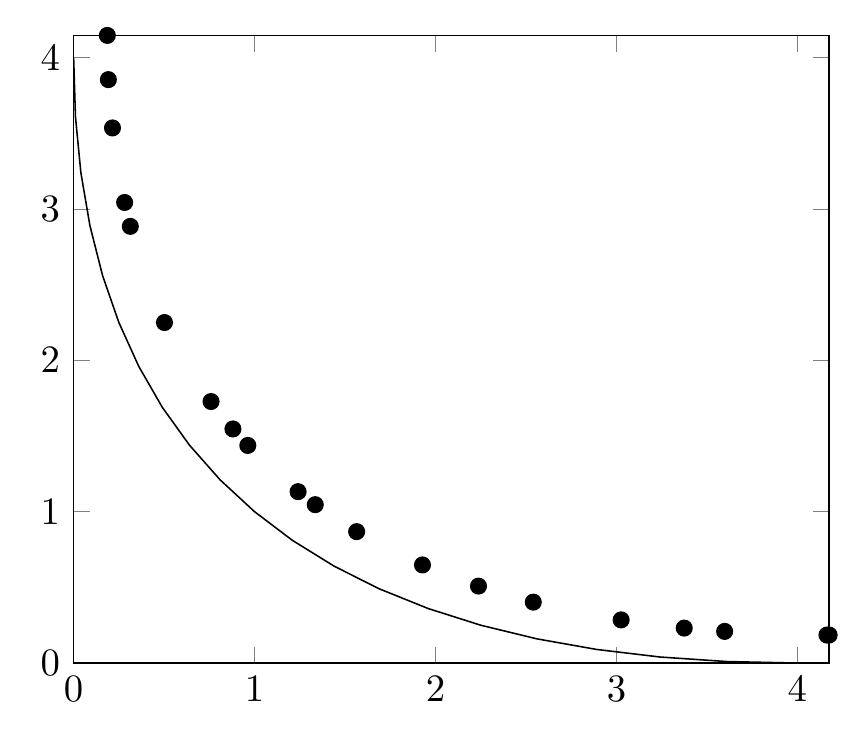
\begin{tikzpicture}[scale=1.4]
        \begin{axis}[enlargelimits=false]
            \addplot [] coordinates {
                (0.000000,4.000000) (0.010000,3.610000) (0.040000,3.240000) (0.090000,2.890000) (0.160000,2.560000) (0.250000,2.250000) (0.360000,1.960000) (0.490000,1.690000) (0.640000,1.440000) (0.810000,1.210000) (1.000000,1.000000) (1.210000,0.810000) (1.440000,0.640000) (1.690000,0.490000) (1.960000,0.360000) (2.250000,0.250000) (2.560000,0.160000) (2.890000,0.090000) (3.240000,0.040000) (3.610000,0.010000) (4.000000,0.000000) 
            };
            
            \addplot [only marks] coordinates {
                (4.175365,0.185087) (0.186029,4.147305) (0.759281,1.728098) (0.501946,2.250118) (3.597814,0.209174) (1.927899,0.648381) (0.281815,3.043491) (1.240382,1.132531) (0.962549,1.437914) (3.374370,0.231054) (1.564048,0.868335) (2.237433,0.508459) (0.214605,3.535965) (4.163266,0.185209) (1.335301,1.046529) (0.191885,3.855241) (2.540124,0.402521) (3.025805,0.285244) (0.880308,1.546811) (0.313213,2.885489) 
 
            };
        \end{axis}
    \end{tikzpicture}
\end{figure}